\documentclass{beamer}

\usetheme{Warsaw}
\usecolortheme{beaver}
% \usecolortheme{spruce}
\useoutertheme{infolines}
% \usetheme{Montpellier}

\title[TECE progress meeting]{TECE progress meeting}
\author[RJC Bilderbeek]{Rich\`{e}l JC Bilderbeek}
\institute[University of Groningen]{University of Groningen}
\date[2017-09-13]{2017-09-13}
\subject{Phylogenetics}

\AtBeginSection[]
{
  \begin{frame}
    \frametitle{Table of Contents}
    \tableofcontents[currentsection]
  \end{frame}
}

\titlegraphic{
  
\includegraphics[width=\textwidth,width=.18\textwidth]{rug_logo_big.png}
  \hspace*{0.05in}
  
\includegraphics[width=\textwidth,width=.50\textwidth]{gelifes-header-690x220.png}
  \hspace*{0.05in}
  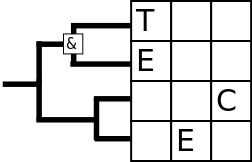
\includegraphics[width=\textwidth,width=.25\textwidth]{tece_logo_2.png}
}

%%%%%%%%%%%%%%%%%%%%%%%%%%%%%%%%%%%%%%%%%%%%%%%%%%%%%%%%%%%%%%%%%%%%%%%%%%%%%%%%
% References
%%%%%%%%%%%%%%%%%%%%%%%%%%%%%%%%%%%%%%%%%%%%%%%%%%%%%%%%%%%%%%%%%%%%%%%%%%%%%%%%
% Don't. Add references as footnotes instead...
%%%%%%%%%%%%%%%%%%%%%%%%%%%%%%%%%%%%%%%%%%%%%%%%%%%%%%%%%%%%%%%%%%%%%%%%%%%%%%%%
\begin{document}

\frame{\titlepage}

%\begin{frame}
%\frametitle{Table of Contents}
%\tableofcontents[currentsection]
%\end{frame}

\section[Section]{Introduction}

%%%%%%%%%%%%%%%%%%%%%%%%%%%%%%%%%%%%%%%%%%%%%%%%%%%%%%%%%%%%%%%%%%%%%%%%%%%%%%%%
\begin{frame}
  \frametitle[]{Tree of life\footnotemark}
  \begin{columns}[T]
    \begin{column}{.45\textwidth}
      \begin{block}{}
        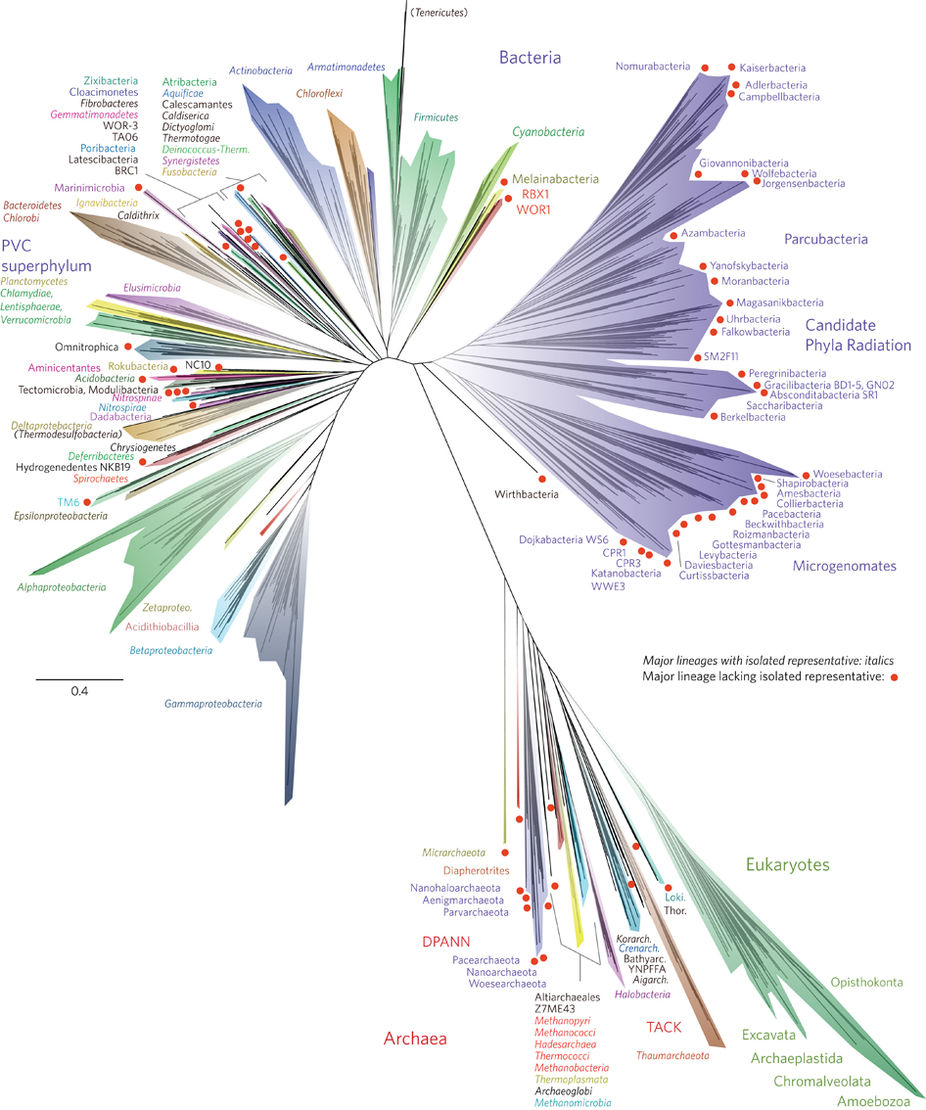
\includegraphics[height=0.65\textheight]{tree_of_life_2016.jpg}
      \end{block}
    \end{column}
    \begin{column}{.5\textwidth}
      \begin{block}{}
        Uses RAxML\footnotemark
      \end{block}
    \end{column}
  \end{columns}
  \footnotetext[1]{Stamatakis, Alexandros. 2014. Bioinformatics 30.9 (2014).}
  \footnotetext[2]{Hug, Laura A., et al. 2016. Nature Microbiology 1 (2016).}
  %\footnotetext[1]{Stamatakis, Alexandros. "RAxML version 8: a tool for phylogenetic analysis and post-analysis of large phylogenies." Bioinformatics 30.9 (2014): 1312-1313.}
  %\footnotetext[2]{Hug, Laura A., et al. "A new view of the tree of life." Nature Microbiology 1 (2016): 16048.}
\end{frame}
%%%%%%%%%%%%%%%%%%%%%%%%%%%%%%%%%%%%%%%%%%%%%%%%%%%%%%%%%%%%%%%%%%%%%%%%%%%%%%%%




%%%%%%%%%%%%%%%%%%%%%%%%%%%%%%%%%%%%%%%%%%%%%%%%%%%%%%%%%%%%%%%%%%%%%%%%%%%%%%%%
\begin{frame}
  \frametitle{New giraffe species ... \footnotemark\footnotemark}
  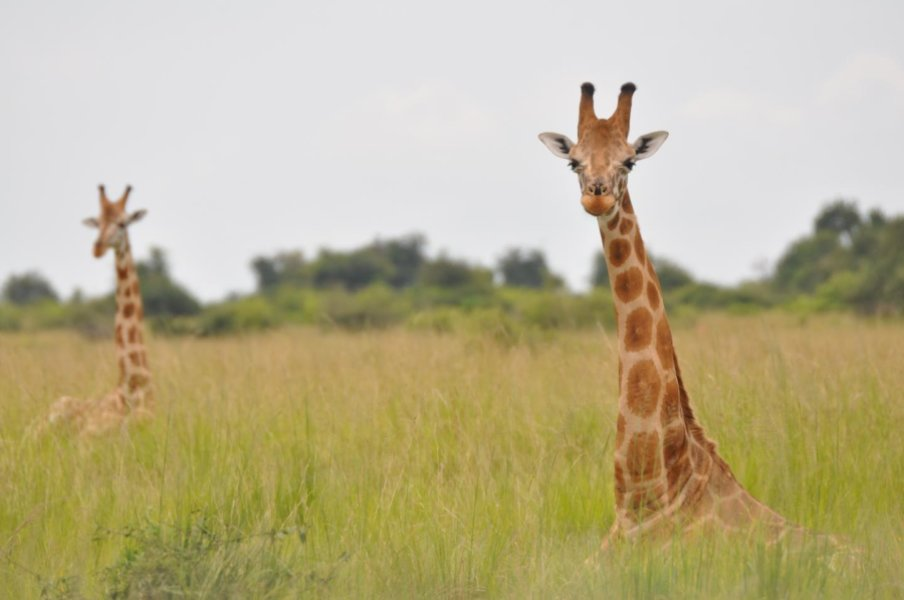
\includegraphics[height=0.8\textheight]{fennessy_2016_nubian_giraffe.jpg}
  \footnotetext[3]{Fennessy, Julian, et al. 2016. Current Biology 26.18.}
  \footnotetext[4]{Picture by Julian Fennessy}
  %\footnotetext[3]{Fennessy, Julian, et al. "Multi-locus analyses reveal four giraffe species instead of one." Current Biology 26.18 (2016): 2543-2549.}
  %\footnotetext[4]{Picture by Julian Fennessy}
\end{frame}
%%%%%%%%%%%%%%%%%%%%%%%%%%%%%%%%%%%%%%%%%%%%%%%%%%%%%%%%%%%%%%%%%%%%%%%%%%%%%%%%

%%%%%%%%%%%%%%%%%%%%%%%%%%%%%%%%%%%%%%%%%%%%%%%%%%%%%%%%%%%%%%%%%%%%%%%%%%%%%%%%
\begin{frame}
  \frametitle{... for quite some time\footnotemark}
  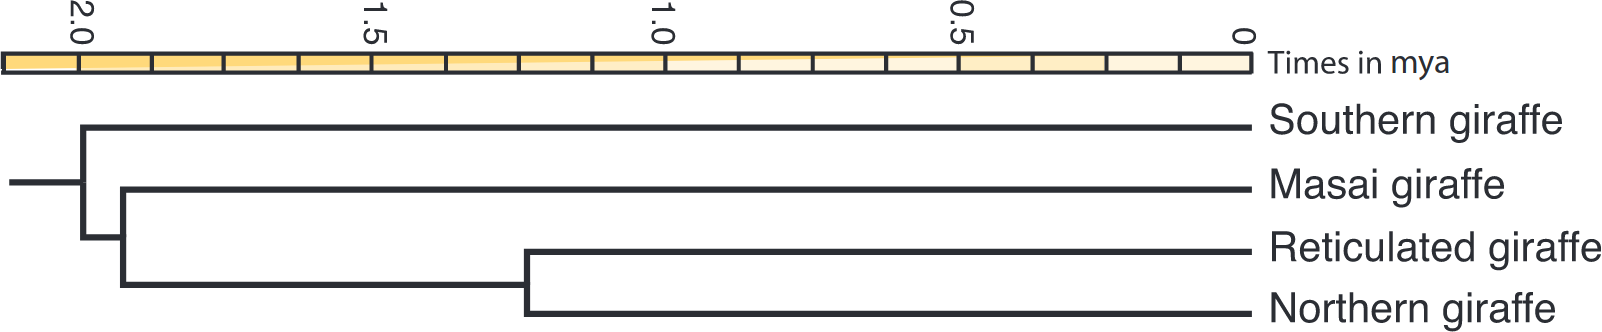
\includegraphics[width=\textwidth]{fennessy_2016_tree.png}
  \footnotetext[5]{Fennessy, Julian, et al. 2016. Current Biology 26.18.}
  % \footnotetext[5]{Fennessy, Julian, et al. "Multi-locus analyses reveal four giraffe species instead of one." Current Biology 26.18 (2016): 2543-2549.}
\end{frame}
%%%%%%%%%%%%%%%%%%%%%%%%%%%%%%%%%%%%%%%%%%%%%%%%%%%%%%%%%%%%%%%%%%%%%%%%%%%%%%%%

\section[Section]{Research question}

%%%%%%%%%%%%%%%%%%%%%%%%%%%%%%%%%%%%%%%%%%%%%%%%%%%%%%%%%%%%%%%%%%%%%%%%%%%%%%%%
\begin{frame}
  \frametitle{Research question}

  What if ...
\end{frame}
%%%%%%%%%%%%%%%%%%%%%%%%%%%%%%%%%%%%%%%%%%%%%%%%%%%%%%%%%%%%%%%%%%%%%%%%%%%%%%%%

\end{document}